\documentclass{article}
\usepackage{tikz}
\usetikzlibrary{shapes,arrows,shadows}
% Define the layers to draw the diagram
\pgfdeclarelayer{background}
\pgfdeclarelayer{foreground}
\pgfsetlayers{background,main,foreground}
\tikzstyle{sensor}=[draw, fill=blue!20, text width=5em, 
    text centered, minimum height=2.5em,drop shadow]
\tikzstyle{ann} = [above, text width=5em, text centered]
\tikzstyle{wa} = [sensor, text width=10em, fill=red!20, 
    minimum height=6em, rounded corners, drop shadow]
\tikzstyle{sc} = [sensor, text width=13em, fill=red!20, 
    minimum height=10em, rounded corners, drop shadow]
\tikzstyle{sc2} = [sensor, text width=13em, fill=green!20, 
    minimum height=5em, rounded corners, drop shadow]
\tikzstyle{sc3} = [sensor, text width=13em, fill=blue!20, 
    minimum height=5em, rounded corners, drop shadow]
\tikzstyle{sc4} = [sensor, text width=5em, fill=red!20, 
    minimum height=5em, drop shadow]
\tikzstyle{sc5} = [sensor, text width=5em, fill=red!20, dashed, 
    minimum height=5em, drop shadow]
\tikzstyle{sc6} = [sensor, text width=5em, fill=purple!80, 
    minimum height=5em, drop shadow]   
\begin{document}
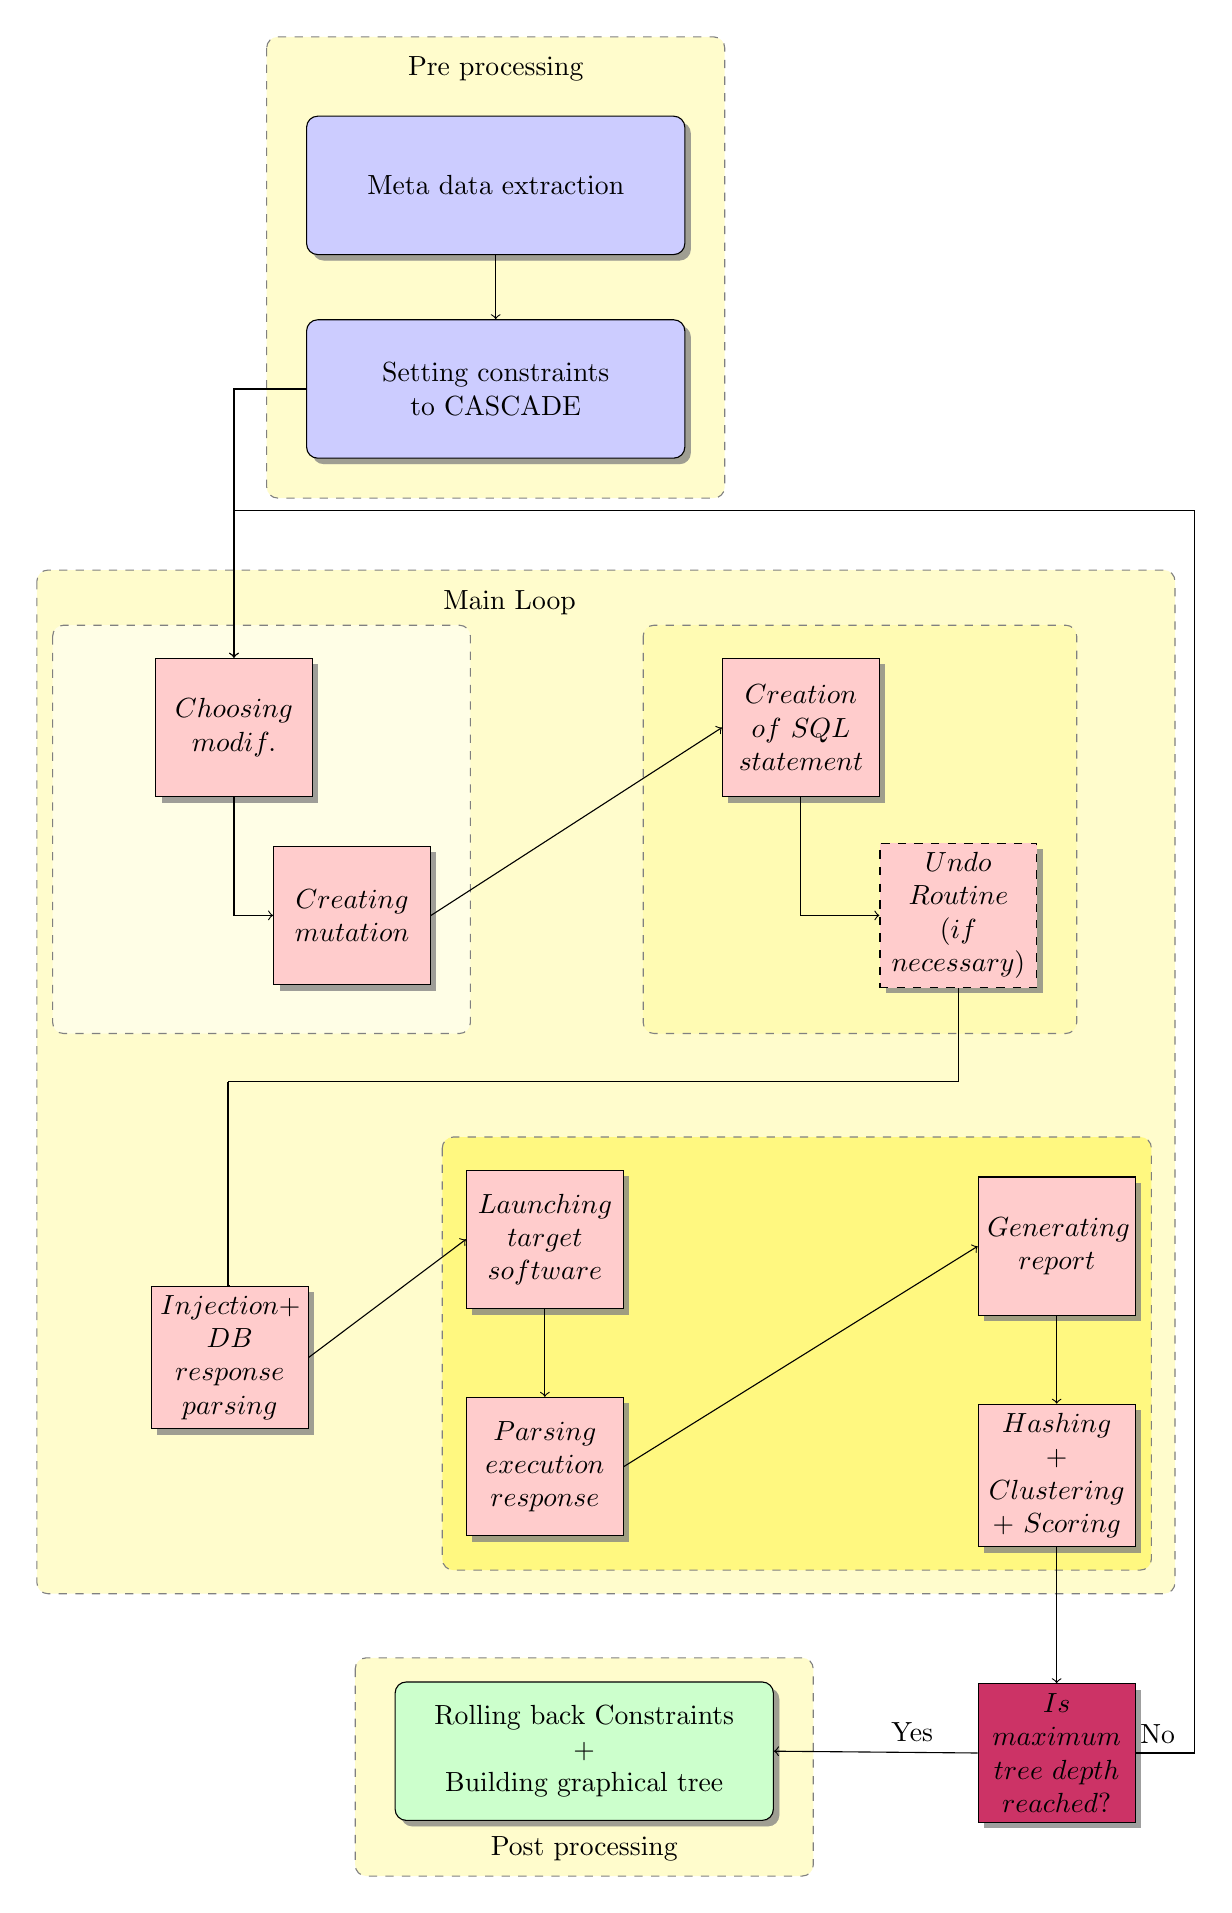
\begin{tikzpicture}
    \node (wa)[sc3]  {Meta data extraction};
    \path (wa.south)+(0,-1.7) node (wa2)[sc3] {Setting constraints to CASCADE};
   
               
    \path (wa.north) +(0,0.6) node (asrs) {Pre processing};
  
    \begin{pgfonlayer}{background}
        \path (wa.west |- wa.north)+(-0.5,1) node (a) {};
        \path (wa2.east |- wa2.south)+(+0.5,-0.5) node (c) {};
          
        \path[fill=yellow!20,rounded corners, draw=black!50, dashed]
            (a) rectangle (c);           
            
    \end{pgfonlayer}
   
    \path (wa.south)+(3,-7.5) node (syscomb) {};
    \path (syscomb.west)+(-6.2,1.5) node (asrt1) [sc4] {$Choosing$ $modif.$};
    \path (asrt1.south)+(1.5,-1.5) node (asrt4) [sc4] {$Creating$ $mutation$};
    \path (syscomb.west)+(1,1.5) node (asrt2)[sc4] {$Creation$ $of$ $SQL$ $statement$};
    \path (asrt2.south)+(2,-1.5) node (asrt5)[sc5] {$Undo$ $Routine$ $(if$ $necessary)$};
    \path (syscomb.east)+(4,-8) node (asrt3)[sc4] {$Hashing$ + $Clustering$ \\ + $Scoring$};
    \path (syscomb.east)+(-2.5,-5) node (asrt6)[sc4] {$Launching$ $target$ $software$};
    \path (asrt6.south)+(0,-2) node (asrt7)[sc4] {$Parsing$ $execution$ \\ $response$};
    \path (asrt3.north)+(0,2) node (asrt8)[sc4] {$Generating$ $report$};
    \path (asrt6.west)+(-3,-1.5) node (asrt9)[sc4] {$Injection +$ \\ $DB$ $response$ \\ $parsing$};                
          
    \begin{pgfonlayer}{background}
        \path (asrt1.west)+(-1.5,2) node (g) {};
        \path (asrt3.east)+(0.5,-1.5) node (h) {};
         
        \path[fill=yellow!20,rounded corners, draw=black!50, dashed]
            (g) rectangle (h);
    \end{pgfonlayer}    
    
    \begin{pgfonlayer}{background}
        \path (asrt1.west)+(-1.3,1.3) node (g) {};
        \path (asrt4.east)+(0.5,-1.5) node (h) {};
         
        \path[fill=yellow!10,rounded corners, draw=black!50, dashed]
            (g) rectangle (h);
    \end{pgfonlayer}    
    
    
    \begin{pgfonlayer}{background}
        \path (asrt2.west)+(-1,1.3) node (g) {};
        \path (asrt5.east)+(0.5,-1.5) node (h) {};
                 
        \path[fill=yellow!30,rounded corners, draw=black!50, dashed]
            (g) rectangle (h);
    \end{pgfonlayer}    
    
	
    \begin{pgfonlayer}{background}
        \path (asrt6.west)+(-0.3,1.3) node (g) {};
        \path (asrt3.east)+(0.2,-1.2) node (h) {};
         
        \path[fill=yellow!50,rounded corners, draw=black!50, dashed]
            (g) rectangle (h);
    \end{pgfonlayer}    
    
    \path (asrt1.north) + (3.5,0.7) node (asrs) {Main Loop};
        
    \path (syscomb.east)+(-2.0,-11.5) node (block3) [sc2] {Rolling back Constraints \\ + \\ Building graphical tree};    
   
  
    \begin{pgfonlayer}{background}
        \path (block3.west |- block3.north)+(-0.5,0.3) node (a) {};
        \path (block3.east |- block3.south)+(+0.5,-0.7) node (c) {};
          
        \path[fill=yellow!20,rounded corners, draw=black!50, dashed]
            (a) rectangle (c);           
           
            
    \end{pgfonlayer}
    
        \path (block3.south) +(-0,-0.35) 
        node (block3Legend) {Post processing};    

	%%% arrows
    \path (syscomb.south)+(-6.4,-3) node (pos) {};
    \path (asrt2.north)+(5,2) node (pos2) {};
    \path (asrt3.south)+(0,-2.61) node (check) [sc6] {$Is$ $maximum$ $tree$ $depth$ $reached?$};
	
	\path [draw, ->] (wa.south) -- (wa2.north) {} ;
    \path [draw, ->] (wa2.west) -| (asrt1.north) {}; 
    \path [draw, ->] (asrt1.south) |- (asrt4.west) {}; 
    \path [draw, ->] (asrt4.east) -- (asrt2.west) {};
    \path [draw, ->] (asrt2.south) |- (asrt5.west) {};
    \path [draw, -] (asrt5.south) |- (pos.north) {};
    \path [draw, -] (pos.north) |- (asrt9.north) {};
    \path [draw, ->] (asrt9.east) -- (asrt6.west) {};
    \path [draw, ->] (asrt6.south) -- (asrt7.north) {};
    \path [draw, ->] (asrt7.east) -- (asrt8.west) {};
    \path [draw, ->] (asrt8.south) -- (asrt3.north) {};
    \path [draw, ->] (asrt3.south) -- (check.north) {};
    \path [draw, ->] (check.west) -- (block3.east) node [above,xshift=50] {Yes};
    \path [draw, -] (check.east) node [above,xshift=8] {No} -| (pos2.south) {};
    \path [draw, ->] (pos2.south) -| (asrt1.north) {};

\end{tikzpicture}
\end{document}
